\documentclass[
	10pt,								% globale Schriftgröße
	parskip=half-,						% setzt Absatzabstand hoch
	paper=a4,							% Format
	english,ngerman,					% lädt Sprachpakete
	]{scrartcl}							% Dokumentenklasse

% //////////////////// Pakete laden ////////////////////
\usepackage{amsmath}			% MUSS vor fontspec geladen werden
\usepackage{mathtools}			% modifiziert amsmath
\usepackage{amssymb}			% mathematische symbole, für \ceckmarks
\usepackage{amsthm}				% für proof
\usepackage{mathrsfs}			% für \mathscr
\usepackage{latexsym}
\usepackage{marvosym}				% für Lightning

\usepackage{fontspec} 			% funktioniert nur mit den neueren Compilern z.B. XeLaTeX
\usepackage{microtype}			% für bessere Worttrennung
\usepackage[ngerman]{babel} 	% Spracheinstellung
\usepackage{csquotes}
\usepackage{lmodern}			% verändert verwendete Schriftart, damit sie weniger pixelig ist

\usepackage{verbatim}
\usepackage{listings}			% Für Quellcode

\usepackage{graphicx}
\usepackage{tabularx}			% für Tabellen mit gleicher Spaltenbreite und automatischen Umbrüchen
\usepackage{fullpage}
\usepackage{multirow}			% für multirow in tabulars
\usepackage{rotate}
\usepackage[cmyk,table]{xcolor} % um Farben zu benutzen, kann mehr als das Paket color
\usepackage[					% Verlinkungen
	colorlinks,					% farbige Schrift, statt farbiger Rahmen
	linktocpage,				% verlinkt im Abb.Verzeichnis Seitenzahl statt Bildunterschrift
	linkcolor=blue				% setzt Farbe der Links auf blau
	]{hyperref}					% nur für digitale Anwendungen, url = "http://www.example.com"
\usepackage{url}				% für Webadressen wie e-mail usw.: "\url{http://www.example.com}"

\usepackage{enumerate}			% für versch. Aufzählungezeichen wie z.B. a)
\usepackage{xspace}				% folgt ein Leerzeichen nach einem \Befehl, wird es nicht verschluckt.
\usepackage{cancel}				% für das Durchstreichen u.a. in Matheformeln mit \cancel
\usepackage{float}              % zum Forcieren der Position von figure-Umgebungen

% zum Zeichnen (u.a. von Graphen)
\usepackage{fp}
\usepackage{tikz}
\usetikzlibrary{tikzmark}			% für \tikzmark{toRemember}
\usetikzlibrary{positioning}	% verbesserte Positionierung der Knoten
\usetikzlibrary{automata}		% für Automaten (GTI)
\usetikzlibrary{arrows}
\usetikzlibrary{shapes}
\usetikzlibrary{decorations.pathmorphing}
\usetikzlibrary{decorations.pathreplacing}
\usetikzlibrary{decorations.shapes}
\usetikzlibrary{decorations.text}

% //////////////////// Syntaxhighlighting ////////////////////
\lstloadlanguages{Python, Haskell, [LaTeX]TeX, Java}
\lstset{
   basicstyle=\footnotesize\ttfamily,	% \scriptsize the size of the fonts that are used for the code
   backgroundcolor = \color{bgcolour},	% legt Farbe der Box fest
   breakatwhitespace=false,	% sets if automatic breaks should only happen at whitespace
   breaklines=true,			% sets automatic line breaking
   captionpos=t,				% sets the caption-position to bottom, t for top
   commentstyle=\color{codeblue}\ttfamily,% comment style
   frame=single,				% adds a frame around the code
   keepspaces=true,			% keeps spaces in text, useful for keeping indentation
							% of code (possibly needs columns=flexible)
   keywordstyle=\bfseries\ttfamily\color{codepurple},% keyword style
   numbers=left,				% where to put the line-numbers;
   							% possible values are (none, left, right)
   numberstyle=\tiny\color{codegreen},	% the style that is used for the line-numbers
   numbersep=5pt,			% how far the line-numbers are from the code
   stepnumber=1,				% nummeriert nur jede i-te Zeile
   showspaces=false,			% show spaces everywhere adding particular underscores;
							% it overrides 'showstringspaces'
   showstringspaces=false,	% underline spaces within strings only
   showtabs=false,			% show tabs within strings adding particular underscores
   flexiblecolumns=false,
   tabsize=1,				% the step between two line-numbers. If 1: each line will be numbered
   stringstyle=\color{orange}\ttfamily,	% string literal style
   numberblanklines=false,				% leere Zeilen werden nicht mitnummeriert
   xleftmargin=1.2em,					% Abstand zum linken Layoutrand
   xrightmargin=0.4em,					% Abstand zum rechten Layoutrand
   aboveskip=2ex, 
}

\lstdefinestyle{py}{
   language=Python,
}
\lstdefinestyle{hs}{
   language=Haskell,
}
\lstdefinestyle{tex}{
	language=[LaTeX]TeX,
	escapeinside={\%*}{*)},     % if you want to add LaTeX within your code
	texcsstyle=*\bfseries\color{blue},% hervorhebung der tex-Schlüsselwörter
	morekeywords={*,$,\{,\},\[,\],lstinputlisting,includegraphics,
	rowcolor,columncolor,listoffigures,lstlistoflistings,
	subsection,subsubsection,textcolor,tableofcontents,colorbox,
	fcolorbox,definecolor,cellcolor,url,linktocpage,subtitle,
	subject,maketitle,usetikzlibrary,node,path,addbibresource,
	printbibliography},% if you want to add more keywords to the set
     numbers=none,
     numbersep=0pt,
     xleftmargin=0.4em,
}

\lstdefinestyle{java}{
	language=Java,
	extendedchars=true,		% lets you use non-ASCII characters;
   						% for 8-bits encodings only, does not work with UTF-8
}

\lstdefinelanguage[x64]{Assembler}     % add a "x64" dialect of Assembler
   [x86masm]{Assembler} % based on the "x86masm" dialect
   % with these extra keywords:
   {morekeywords={CDQE,CQO,CMPSQ,CMPXCHG16B,JRCXZ,LODSQ,MOVSXD, %
                  POPFQ,PUSHFQ,SCASQ,STOSQ,IRETQ,RDTSCP,SWAPGS, %
                  rax,rdx,rcx,rbx,rsi,rdi,rsp,rbp, %
                  r8,r8d,r8w,r8b,r9,r9d,r9w,r9b}
}					% for 8-bits encodings only, does not work with UTF-8

\lstdefinestyle{c}{
	language=c,
	extendedchars=true,		% for 8-bits encodings only, does not work with UTF-8
}

% //////////////////// eigene Kommandos ////////////////////
\newcommand\FU{Freie Universität Berlin\xspace}% benötigt package xspace
\newcommand\gdw{g.\,d.\,w.\xspace}
\newcommand\oBdA{o.\,B.\,d.\,A.\xspace}
\newcommand{\Eu}{\texteuro}
\newcommand\N{\mathbb{N}\xspace}
\newcommand\Q{\mathbb{Q}\xspace}
\newcommand\R{\mathbb{R}\xspace}
\newcommand\Z{\mathbb{Z}\xspace}
\newcommand\ohneNull{\ensuremath{\backslash\lbrace 0\rbrace}}% \{0}
\let\dhALT\dh	% Schreibt Befehl \dh in \dhALT um
\renewcommand\dh{d.\,h.\xspace}	%renew überschreibt command \dh
\newcommand\Bolt{\;\text{\LARGE\raisebox{-0.3em}{\Lightning}\normalsize}\xspace}% Blitz
\newcommand\zz{\ensuremath{\raisebox{+0.25ex}{Z}% zu zeigen
			\kern-0.4em\raisebox{-0.25ex}{Z}%
			\;\xspace}}
\newcommand{\from}{\ensuremath{\colon}}
\newcommand{\floor}[1]{\lfloor{#1}\rfloor}
\newcommand{\ceil}[1]{\lceil{#1}\rceil}
 \renewcommand{\L}{\ensuremath{\mathcal{L}}\xspace}
 \renewcommand{\P}{\ensuremath{\mathcal{P}}\xspace}
 \newcommand{\NL}{\ensuremath{\mathcal{N}\kern-0.2em\mathcal{L}}\xspace}
 \newcommand{\NP}{\ensuremath{\mathcal{NP}}\xspace}

% //////////////////// Mathefunktionen ////////////////////
\DeclareMathOperator{\Landau}{\mathcal{O}}
\DeclareMathOperator{\True}{True}
\DeclareMathOperator{\False}{False}

% //////////////////// eigene Theoreme ////////////////////
\newtheorem{theorem}{Satz}
\newtheorem{corollary}[theorem]{Folgerung}
\newtheorem{lemma}[theorem]{Lemma}
\newtheorem{observation}[theorem]{Beobachtung}
\newtheorem{definition}[theorem]{Definition}
\newtheorem{Literatur}[theorem]{Literatur}
% konfiguriert proof
\makeatletter
\newenvironment{Proof}[1][\proofname]{\par
  \pushQED{\qed}%
  \normalfont \topsep6\p@\@plus6\p@\relax
  \trivlist
  \item[\hskip\labelsep
%         \itshape
        \bfseries
    #1\@addpunct{.}]\ignorespaces
}{%
  \popQED\endtrivlist\@endpefalse
}
\makeatother

% //////////////////// eigene Farben ////////////////////
\let\definecolor=\xdefinecolor
\definecolor{FUgreen}{RGB}{153,204,0}
\definecolor{FUblue}{RGB}{0,51,102}

\definecolor{middlegray}{rgb}{0.5,0.5,0.5}
\definecolor{lightgray}{rgb}{0.8,0.8,0.8}
\definecolor{orange}{rgb}{0.8,0.3,0.3}
\definecolor{azur}{rgb}{0,0.7,1}
\definecolor{yac}{rgb}{0.6,0.6,0.1}
\definecolor{Pink}{rgb}{1,0,0.6}

\definecolor{bgcolour}{rgb}{0.97,0.97,0.97}
\definecolor{codegreen}{rgb}{0,0.6,0}
\definecolor{codegray}{rgb}{0.35,0.35,0.35}
\definecolor{codepurple}{rgb}{0.58,0,0.82}
\definecolor{codeblue}{rgb}{0.4,0.5,1}

% //////////////////// eigene Settings ////////////////////

\textheight = 230mm		% Höhe des Satzspiegels / Layouts
\footskip = 10ex			% Abstand zw. Fußzeile und Grundlinie letzter Textzeile
\parindent 0pt			% verhindert Einrückung der 1. Zeile eines Absatzes
\setkomafont{sectioning}{\rmfamily\bfseries}% setzt Ü-Schriften in Serifen, {disposition}
\graphicspath{ {./src/} } 
\usepackage{hyperref}

\newcommand{\dozent}{Volker Roth}
\newcommand{\tutor}{Oliver Wiese}
\newcommand{\tutoriumNo}{02\\Materialien: Latex, VSC, Skript}
\newcommand{\ubungNo}{06}
\newcommand{\veranstaltung}{Rechnersicherheit}
\newcommand{\semester}{SoSe 21}

% /////////////////////// BEGIN DOKUMENT /////////////////////////
\begin{document}
% /////////////////////// BEGIN TITLEPAGE /////////////////////////
\begin{titlepage}
	\subject{\dozent}
	\title{\veranstaltung, \semester}
	\subtitle{\Large Übung \ubungNo\\ \large\vspace{1ex} TutorIn: \tutor\\ Tutorium \tutoriumNo}
	\author{\studenten}
	\date{\normalsize \today}
\end{titlepage}

\maketitle								% Erstellt das Titelblatt
\vspace*{-10cm}							% rückt Logo an den oberen Seitenrand
\makebox[\dimexpr\textwidth+1cm][r]{	%rechtsbündig und geht rechts 1cm über Layout hinaus
	
\includegraphics[width=0.4\textwidth]{src/fu_logo} % fügt FU-Logo ein
}
% /////////////////////// END TITLEPAGE /////////////////////////

\vspace{7cm}							% Abstand
\rule{\linewidth}{0.8pt}				% horizontale Linie

% /////////////////////// Task 1 /////////////////////////
\section{Password Generation using Context Free Grammars}
\begin{itemize}

    % /////////////////////// a /////////////////////////
    \item {\itshape Consider the following probabilistic context-free grammar.}
    
    {\Large
    \begin{tabular}{c|c}
        \textbf{Production rule} & \textbf{Probability}\\ 
        \hline  
        S \xrightarrow{} D_1L_3S_2D_1 & 0.75 \\
        S \xrightarrow{} L_3D_1S_1 & 0.25 \\
        \hline  
        D_1 \xrightarrow{} 4 & 0.60 \\
        D_1 \xrightarrow{} 5 & 0.20 \\
        D_1 \xrightarrow{} 6 & 0.20 \\
        \hline  
        S_1 \xrightarrow{} ! & 0.65 \\
        S_1 \xrightarrow{} \% & 0.30 \\
        S_1 \xrightarrow{} \# & 0.05 \\
        \hline 
        S_2 \xrightarrow{} \$\$ & 0.70 \\
        S_2 \xrightarrow{} ** & 0.30 \\
    \end{tabular}
    }
    
    \item {\itshape and the following priority queue:}
    
    {\Large
    \begin{tabular}{c|c|c|c}
        \textbf{Base Struct} & \textbf{Pre-Terminal} & \textbf{Probability} & \textbf{Pivot Value}\\ 
        \hline  
        \textcolor{blue}{D}_1^{\textcolor{red}{0}} L_3 S_2^{\textcolor{red}{0}} D_1^{\textcolor{red}{0}} & 4L_3\$\$4 & 0.188 & \textcolor{blue}{0} \\
        
        L_3\textcolor{blue}{D}_1^{\textcolor{red}{0}} S_1^{\textcolor{red}{0}} & L_34! & 0.097 & \textcolor{blue}{0} \\
    \end{tabular}
    }  
    
\end{itemize} 
   
\newpage
\begin{enumerate}[(a)]
    \item {\itshape Calculate the next five pre-terminal structures that the enumerator (as discussed in class)does output and the resulting priority queue.}
    \begin{enumerate}[1.]
        \item After the first password was extracted:
        
        {\Large
        \begin{tabular}{c|c|c|c}
            \textbf{Base Struct} & \textbf{Pre-Terminal} & \textbf{Probability} & \textbf{Pivot Value}\\ 
            \hline  
            
            L_3\textcolor{blue}{D}_1^{\textcolor{red}{0}} S_1^{\textcolor{red}{0}} & L_34! & 0.097 & \textcolor{blue}{0} \\
            
            D_1^{\textcolor{red}{0}} L_3 \textcolor{blue}{S}_2^{\textcolor{red}{1}} D_1^{\textcolor{red}{0}} & 4L_3**4 & 0.081 & \textcolor{blue}{1} \\
            
            \textcolor{blue}{D}_1^{\textcolor{red}{1}} L_3 S_2^{\textcolor{red}{0}} D_1^{\textcolor{red}{0}} & 5L_3\$\$4 & 0.063 & \textcolor{blue}{0} \\
            
            D_1^{\textcolor{red}{0}} L_3 S_2^{\textcolor{red}{0}} \textcolor{blue}{D}_1^{\textcolor{red}{1}} & 4L_3\$\$5 & 0.063 & \textcolor{blue}{2} \\
        \end{tabular}
        }  
        
        \item After the second password was extracted:
        
        {\Large
        \begin{tabular}{c|c|c|c}
            \textbf{Base Struct} & \textbf{Pre-Terminal} & \textbf{Probability} & \textbf{Pivot Value}\\ 
            \hline  
            
            D_1^{\textcolor{red}{0}} L_3 \textcolor{blue}{S}_2^{\textcolor{red}{1}} D_1^{\textcolor{red}{0}} & 4L_3**4 & 0.081 & \textcolor{blue}{1} \\
            
            \textcolor{blue}{D}_1^{\textcolor{red}{1}} L_3 S_2^{\textcolor{red}{0}} D_1^{\textcolor{red}{0}} & 5L_3\$\$4 & 0.063 & \textcolor{blue}{0} \\
            
            D_1^{\textcolor{red}{0}} L_3 S_2^{\textcolor{red}{0}} \textcolor{blue}{D}_1^{\textcolor{red}{1}} & 4L_3\$\$5 & 0.063 & \textcolor{blue}{2} \\
            
            L_3 D_1^{\textcolor{red}{0}} \textcolor{blue}{S}_1^{\textcolor{red}{1}} & L_34\% & 0.045 & \textcolor{blue}{1} \\
            
            L_3\textcolor{blue}{D}_1^{\textcolor{red}{1}} S_1^{\textcolor{red}{0}} & L_35! & 0.0325 & \textcolor{blue}{0} \\
        \end{tabular}
        }  
        
    \end{enumerate}
    
    
\end{enumerate}


\newpage
% /////////////////////// Task 2 /////////////////////////
\section{Code Review}
{\itshape Review and test the Python code of your peers. Your focus should be the implementation of the password-based authentication and consider at least the following aspects:}
\begin{enumerate}[1.]
    % /////////////////////// Peer 1 /////////////////////////
    \item \textbf{Peer}:
    \begin{enumerate}[(a)]
        % /////////////////////// a /////////////////////////
        \item {\itshape Used hash function and configuration.}
        
        \textbf{Implemented}
        \lstinputlisting[language=python, linerange={143-145}, firstnumber = 143]{src/u6/user_manager.py}
        
        % /////////////////////// b /////////////////////////
        \item {\itshape Usage and generation of salts and randomness.}
        
        \textbf{Implemented}
        \lstinputlisting[language=python, linerange={188-197}, firstnumber=188]{src/u6/user_manager.py}

        % /////////////////////// c /////////////////////////
        \item {\itshape Duplicate user names.}
        
        \textbf{Prevented}
        \lstinputlisting[language=python, linerange={41-48, 52-57}, firstnumber=41]{src/u6/user_manager.py}
\newpage    
        % /////////////////////// d /////////////////////////
        \item {\itshape Simultaneous creation of users with the same name.}
        
        \textbf{Not prevented. Still possible.} I added a sleep in the server, just to demonstrate it, even without the sleep it can happen, as we work with threads. To fix this you can use locks in the server authentication method.
        \lstinputlisting[language=python, linerange={41-57}, firstnumber=41]{src/u6/user_manager.py}
        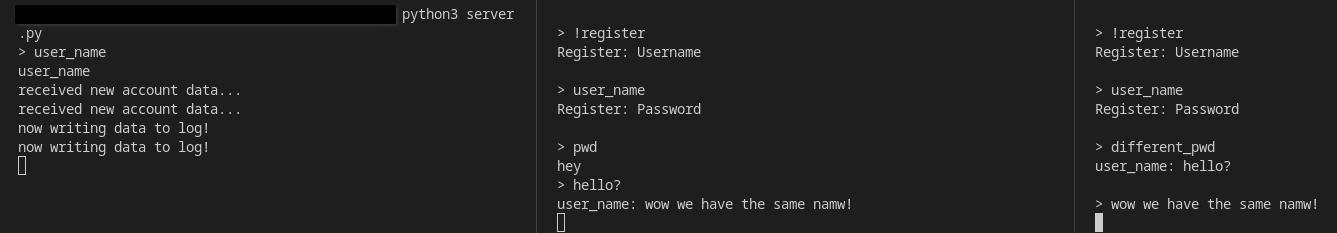
\includegraphics[width=\linewidth]{src/u6/nolock.png}
\newpage
        % /////////////////////// extra /////////////////////////
        \item {\itshape \textbf{Extra:} I was able to find some security risks in your code with bandit.}
        \lstinputlisting[language=python, linerange={9-44}, firstnumber=9]{src/u6/bandit_output_peer_1.txt}
        \begin{itemize}
            \item To fix the first two to security risks you could use the bcrypt module which has a 'safer' hashing function. Here is an example syntax:
            \lstinputlisting[language=python, linerange={1-3}, firstnumber=1]{src/u6/example_1.txt}
            
        \item To fix the third/fourth security risk you would need to create 'real' randomness, which can be done with a quantum PCs, but as you most likely don't have one right now, you can also use the bcrypt module to create a 'safer' salt. With this salt generator bandit will stop throwing an error. Here is the example:
        \lstinputlisting[language=python, linerange={5}, firstnumber=5]{src/u6/example_1.txt}
        \end{itemize}
        
    \end{enumerate}
    
    
    
\newpage
    % /////////////////////// Peer 2 /////////////////////////
    \item \textbf{Peer}:
    \begin{enumerate}[(a)]
        % /////////////////////// a /////////////////////////
        \item {\itshape Used hash function and configuration.}
        
        \textbf{Implemented}
        \lstinputlisting[language=python, linerange={57-57}, firstnumber = 57]{src/u6/server.py}
        
        % /////////////////////// b /////////////////////////
        \item {\itshape Usage and generation of salts and randomness.}
        
        \textbf{Somewhat implemented.} Salt is used but not random!
        \lstinputlisting[language=python, linerange={11-11}, firstnumber=11]{src/u6/server.py}

        % /////////////////////// c /////////////////////////
        \item {\itshape Duplicate user names.}
        
        \textbf{Prevented}
        \lstinputlisting[language=python, linerange={64-71}, firstnumber=64]{src/u6/server.py}
        
        % /////////////////////// d /////////////////////////
        \item {\itshape Simultaneous creation of users with the same name.}
        
        \textbf{Somewhat prevented. Might still be possible.} But I could not test it, because the server does not allow it when multiple clients try to register / login at the same time. This seems more like a bug than a feature. If this would be fixed, simultaneous creation of users with the same name would be possible. To fix this you can use locks.
        Below is a example on how I tried to register with two clients at the same time. I added a print in the client to show the 'error'.
        
        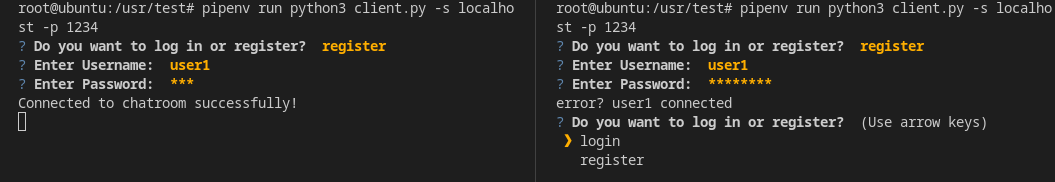
\includegraphics[width=\linewidth]{src/u6/error2.png}
        
        Here is the code snippet of you client. I added the lines 79 and 80.
        \lstinputlisting[language=python, linerange={66-80}, firstnumber=66]{src/u6/client.py}

\newpage
        % /////////////////////// extra /////////////////////////
        \item {\itshape \textbf{Extra:} Bandit found no further security risky.}
        
        % /////////////////////// Error /////////////////////////
        \item {\itshape \textbf{Errors:} I had some errors running your Dockerfile.}
        \begin{itemize}
            \item Your Dockerfile searched for 'client/client.py' and 'server/server.py', but they are named 'server\textbackslash server.py' and 'server\textbackslash server.py'. I fixed it by just renaming them. Here is the log file of the first time I ran your Dockerfile:
            \lstinputlisting[language=python]{src/u6/error.txt}

        \end{itemize}

    \end{enumerate}
    
\end{enumerate}

\end{document}